\documentclass[finnish]{tktltiki2}

% tktltiki2 automatically loads babel, so you can simply
% give the language parameter (e.g. finnish, swedish, english, british) as
% a parameter for the class: \documentclass[finnish]{tktltiki2}.
% The information on title and abstract is generated automatically depending on
% the language, see below if you need to change any of these manually.
% 
% Class options:
% - grading                 -- Print labels for grading information on the front page.
% - disablelastpagecounter  -- Disables the automatic generation of page number information
%                              in the abstract. See also \numberofpagesinformation{} command below.
%
% The class also respects the following options of article class:
%   10pt, 11pt, 12pt, final, draft, oneside, twoside,
%   openright, openany, onecolumn, twocolumn, leqno, fleqn
%
% The default font size is 11pt. The paper size used is A4, other sizes are not supported.
%
% rubber: module pdftex

% --- General packages ---

\usepackage[utf8]{inputenc}
\usepackage[T1]{fontenc}
\usepackage{lmodern}
\usepackage[pdftex]{graphicx}
\usepackage{subfigure}
\usepackage{microtype}
\usepackage{amsfonts,amsmath,amssymb,amsthm,booktabs,color,enumitem,graphicx}
\usepackage[pdftex,hidelinks]{hyperref}

% Automatically set the PDF metadata fields
\makeatletter
\AtBeginDocument{\hypersetup{pdftitle = {\@title}, pdfauthor = {\@author}}}
\makeatother

% --- Language-related settings ---
%
% these should be modified according to your language

% babelbib for non-english bibliography using bibtex
\usepackage[fixlanguage]{babelbib}
\selectbiblanguage{finnish}

% add bibliography to the table of contents
\usepackage[nottoc]{tocbibind}
% tocbibind renames the bibliography, use the following to change it back
\settocbibname{Lähteet}

% --- Theorem environment definitions ---

\newtheorem{lau}{Lause}
\newtheorem{lem}[lau]{Lemma}
\newtheorem{kor}[lau]{Korollaari}

\theoremstyle{definition}
\newtheorem{maar}[lau]{Määritelmä}
\newtheorem{ong}{Ongelma}
\newtheorem{alg}[lau]{Algoritmi}
\newtheorem{esim}[lau]{Esimerkki}

\theoremstyle{remark}
\newtheorem*{huom}{Huomautus}


% --- tktltiki2 options ---
%
% The following commands define the information used to generate title and
% abstract pages. The following entries should be always specified:

\title{Digitaaliset todennukset mobiiliympäristössä}
\author{Taneli Virkkala}
\date{\today}
\level{Kandidaatin tutkielma}
\abstract{Tiivistelmä.}

% The following can be used to specify keywords and classification of the paper:

\keywords{avainsana 1, avainsana 2, avainsana 3}

% classification according to ACM Computing Classification System (http://www.acm.org/about/class/)
% This is probably mostly relevant for computer scientists
% uncomment the following; contents of \classification will be printed under the abstract with a title
% "ACM Computing Classification System (CCS):"
% \classification{}

% If the automatic page number counting is not working as desired in your case,
% uncomment the following to manually set the number of pages displayed in the abstract page:
%
% \numberofpagesinformation{16 sivua + 10 sivua liitteissä}
%
% If you are not a computer scientist, you will want to uncomment the following by hand and specify
% your department, faculty and subject by hand:
%
% \faculty{Matemaattis-luonnontieteellinen}
% \department{Tietojenkäsittelytieteen laitos}
% \subject{Tietojenkäsittelytiede}
%
% If you are not from the University of Helsinki, then you will most likely want to set these also:
%
% \university{Helsingin Yliopisto}
% \universitylong{HELSINGIN YLIOPISTO --- HELSINGFORS UNIVERSITET --- UNIVERSITY OF HELSINKI} % displayed on the top of the abstract page
% \city{Helsinki}
%


\begin{document}

% --- Front matter ---

\frontmatter      % roman page numbering for front matter

\maketitle        % title page
\makeabstract     % abstract page

\tableofcontents  % table of contents

% --- Main matter ---

\mainmatter       % clear page, start arabic page numbering

\section{Johdanto}

% Write some science here.

Digitaalisten allekirjoitusten käyttö on noussut huomattavasti mobiililaitteilla nykypäivänä. Mobiiliympäristössä turvallinen yhteys on varmistettava, koska tietoturvariskit langattomissa verkoissa ovat erittäin suuret \cite{enti}. Teknisen kehityksen ansiosta allekirjoituksia voidaan luoda yleisesti mobiililaitteilla ja parempi tietoturva on mahdollistanut useiden sovellusten käytön. Tietokonelaitteistolla käytettävät protokollat kuten esimerkiksi PKI-malli (julkisen avaimen infrastruktuuri) ovat siirtyneet mobiiliympäristöön sellaisenaan, eivätkä nämä protokollat ole tarvinneet suuria muutoksia toimiakseen. Kehittyneemmän laskentatehon ansiosta monet algoritmit kuten RSA sekä Diffien ja Hellmanin menetelmä ollaan pystytty ottamaan käyttöön kannettavilla laitteilla \cite{enti}. Yhteiseen salaisuuteen perustuva MAC-funktio on myös käytössä tekstiviestien (SMS) lähettämisessä \cite{MAC}. Palvelimille voidaan silti delegoida operaatiot, joita laitteella ei pystytä suorittamaan. Allekirjoitus voidaan luoda tarvittaessa palvelimella tai asiakkaan laitteessa, mutta allekirjoituksen tulee täyttää kaikki sille asetetut ehdot tietoturvaa koskien. Palvelinpohjaisen allekirjoituksen yleensä luo välissä oleva kirjautumispalvelin eikä lopullinen palveluntarjoaja \cite{proxy}.

Digitaalisten allekirjoitusten käyttö mobiiliympäristössä tulisi olla nopeaa ja turvallista. Monet nykyaikaiset sovellukset vaativat jokaisen viestin lähetyksen yhteydessä uuden allekirjoituksen. Esimerkkinä tästä voisi toimia eräänlainen huutokauppasovellus, jossa jokaisen huudon on oltava kiistaton ja todennettu. Lisäksi viestin sisältämän datan tulee olla eheää. \cite{proxy}

Schwabin ja Yangin mukaan \cite{enti} mahdollisia tietoturvariskejä mobiiliympäristössä ovat urkinta, välimieshyökkäys, datan muuntaminen, toisena osapuolena esiintyminen ja laitteen kadottaminen. Mobiililaitteen sisäisen toiminnan ja verkkoviestinnän tulee olla suojattu mahdollisilta riskeiltä. Jos palvelun tarjoajan ja asiakkaan välissä on välityspalvelin, siihen tulee myös muodostaa luotettava yhteys. Koska digitaaliset allekirjoitukset perustuvat julkisen avaimen infrastruktuuriin, on äärimmäisen tärkeää pitää salainen avain mahdollisimman turvassa. Laitteen SIM-kortti on turvallinen paikka säilyttää salaista avainta, joka ei silloin paljastu laitteen käyttöjärjestelmälle. Prosessorin luoma avain paljastuu aina kokonaan laitteelle. Sen sijaan prosessorilla avaimen ja allekirjoituksen luonti on nopeampaa kuin SIM-kortilla \cite{proxy}. 

Varmenne on varmenneviranomaisen tarjoama osa digitaalisen allekirjoituksen luontiin. Varmenneviranomainen on lähettäjästä riippumaton erillinen osapuoli. Jokainen allekirjoitus tarvitsee varmenteen toimiakseen. Viestin lähettäjä liittää varmenteen allekirjoitukseen. \cite{ECC}       


\section{Digitaalisen allekirjoituksen määritelmä}

Digitaalinen allekirjoitus on menetelmä, jolla voidaan todentaa tietyn lähettäjän lähettäneen viestin vastaanottajalle muuttumattomana. Lähettäjä ei voi siis jälkikäteen kiistää lähettämäänsä viestiä (kiistämättömyys). Viesti voi olla lisäksi salattu käyttäen jotain salausmenetelmää kuten esimerkiksi AES-lohkosalausta. Vaikka viestin salaaminen ei suoranaisesti liity digitaaliseen allekirjoitukseen, on salaus tärkeä osa tietoturvaa. Allekirjoitus vaatii toimiakseen tiivistefunktioita ja varmenteen varmenneviranomaiselta. Viesti on siis saapunut oikeana perille, mikäli viestin tiiviste on sama kuin allekirjoitettu tiiviste. Digitaalinen allekirjoitus pohjautuu julkisen avaimen infrastruktuuriin. Mobiiliallekirjoituksella tarkoitetaan digitaalista allekirjoitusta mobiililaitteella.

\subsection{Toiminta} 

Tiivisteistä ja datan eheydestä voidaan todentaa tiedon muuttumattomuus ja lähettäjän kiistämättömyys \cite{moen}. Vastanottaja verifioi viestin allekirjoituksen allekirjoittajan lähettämällä julkisella avaimella eli laskee sanoman tiivisteen ja allekirjoitetun tiivisteen arvon. Molempien arvojen tulisi olla samat, jotta viesti voidaan hyväksyä. Jos viestin sisältöä muutetaan, vastaanottajan avaimella purettu viesti ei ole enää ymmärrettävässä muodossa. Tiivistefunktioita voivat olla SHA-2 ja MD5. On syytä huomata, että SHA-1 ja MD5 ovat jo vanhentuneita tietoturvan kannalta ja uusi standardi SHA-3 on tuloillaan \cite{nist}.   

Viestin varmenteessa on mukana lähettäjän liittämä julkinen avain, jollei sitä ole lähetetty aiemmin. Varmenteen kelpoisuus on varmistettava varmenneviranomaiselta. Myönnetty varmenne on voimassa vain tietyn aikaa. Vastaanottajan on tunnettava kyseinen varmenneviranomainen viestin kelpoisuuden tarkastamiseksi. Lisäksi varmenteen voimassaolo on tarkistettava. Kelpoisuus on siis tarkastettava viranomaisen julkisella avaimella, joka on saatettu lähettää saman viestin mukana. Seuraavien ehtojen on oltava voimassa allekirjoituksessa: uskottavuus, muuttumattomuus, kertakäyttöisyys ja kiistattomuus \cite{e-c}. Digitaalisella allekirjoituksella voidaan siis todentaa vain yksi viesti kerrallaan, ja jokaiselle viestille on luotava uusi allekirjoitus. Menetelmä on yksi turvallisimmista tavoista varmentaa luotettava viestinkulku vastaanottajan ja lähettäjän välillä. Sen sijaan allekirjoitus on raskasta luoda, joten menetelmä vaatii merkittävää laskentatehoa toimiakseen \cite{proxy}. Erityisen vaikeaksi tekee tilanne, jossa salausta joudutaan käyttämään joka palvelimelle siirryttäessä. Digitaalisia allekirjoituksia käytetään siis yleensä yhteydenmuodostuksen aluksi, mutta niistä voidaan luopua myöhemmissä viestien lähteyksissä.

\subsection{Historia}

RSA algoritmina kehitettiin jo vuonna 1977. Ron Rivest, Adi Shamir ja Leonard Adleman \cite{siam} keksivät julkisen avaimen infrastruktuuriin pohjautuvan menetelmän, jossa salaus hoidetaan julkisella avaimella ja viestin purkaminen salaisella avaimella. Tätä salausmuotoa kutsutaan epäsymmetriseksi salaukseksi erillisten avainten takia. Vain vuotta aikaisemmin Diffien ja Hellmanin menetelmä (DH) luotiin Whitfield Diffien ja Martin Hellmanin toimesta. DH perustuu yhteen yhteiseen avaimeen, jolla viestittävät osapuolet voivat salata ja purkaa viestit toisillensa. Käyttötarkoitus on vain erilainen. RSA:ta käytetään digitaalisen allekirjoituksen luontiin, mutta DH perustuu käyttäjien yhteiseen salaisuuteen (symmetrinen salaus) viestin salauksen mahdollistamiseksi. Tämä kyseinen salaisuus DH:ssa voidaan sopia julkisia yhteyksiä pitkin, mutta lopputuloksena vain kaksi osapuolta saavat tietää tämän salaisuuden. DH:ssa viestin salaus ja purku tehdään samalla avaimella, eikä erillistä käyttäjäkohtaista salaista avainta ole.

Vuonna 1988 luotiin tarkat vaatimukset digitaalisille allekirjoituksille. Goldwasserin, Micalin ja Rivestin \cite{siam} mukaan allekirjoitukset eivät saa noudattaa mitään selkeää kaavaa, josta selväkielinen teksti saataisiin yhdistettyä salattuun tekstiin (Chosen Message Attack). Tämä operaatio vaatii julkisen avaimen olevan hallussa ulkopuolisella hyökkääjällä, jota ei saisi tapahtua. DH:n aikana vuonna 1976 oli käytössä takaporttifunktio, joka oli vielä turvattomampi. Jo pelkällä avaimen hallussapidolla pystyi satunnaisella todennäköisyydellä luomaan pätevän tiivisteen viestille. Kaavalla $V =(M,k)$ voitiin lyhyellä viestillä $M$ ja julkisella avaimella $k$ saada arvaamalla verifioitua viesti, jolloin hyökkääjä pääsi lähettämään ja purkamaan yksinkertaisia sanomia.

Internetin laajentuessa ympäri maailmaa 1990-luvun alkupuolella monet sähköiset palvelut yleistyivät. 1993 kehitetty ensimmäinen ohjelmointirajapinta SSL:lle oli alku myös myöhemmin käyttöön tulleelle TLS:lle. Nämä kummatkin protokollat toivat salauksen Internet-yhteyden välillä toimiviin sovelluksiin. Esimerkiksi HTML-sivujen siirrossa voidaan käyttää turvallista HTTPS-protokollaa, jossa data kulkee salatussa muodossa. Salaus ja purku voivat noudattaa PKI-mallia käytettäessä TLS:llää. Suomessa keksitty SSH-protokolla mahdollisti puolestaan etäyhteyden asiakkaan ja palvelimen välillä. Allekirjoitusalgoritmit kuten RSA tulivat tämän kaltaisessa yhteyden muodostuksessa yleisiksi ja salaisella avaimella voitiin korvata salasanat. Nykyisin myös mobiililaitteella voi muodostaa etäyhteyksiä, ja aivan samoja TLS- ja HTTPS-protokollia käytetään osapuolten todennuksissa mobiilisovelluksissa.

2000-luvun alussa digitaaliset allekirjoitukset yleistyivät mobiililaitteissa. WAP-sovellusten (Wireless Application Protocol) tullessa käyttöön digitaalisia todennuksia pystyttiin käyttöönottaa mobiiliympäristössä ja monet yritykset alkoivat todentaa asiakkaitaan mobiiliallekirjoituksilla. Suomessa vasta vuonna 2010 kehitettiin mobiilivarmennejärjestelmä, johon mobiiliverkko-operaattorit lähtivät mukaan \cite{mobiva}. Virossa jo vuonna 2007 käynnistyi M-ID tunnistautuminen, jossa kansalainen pääsee käyttämään sähköisiä palveluita todentamalla henkilöllisyytensä matkapuhelimeltaan \cite{estonia}. 

\subsection{Matemaattisia selityksiä}

Algoritmien tulkinta vaatii pohjaksi tietämystä matemaattisista funktioista. Kongruenssirelaatiolla merkitään monia kaavoja, joissa käytetään modulaarista aritmetiikkaa. Kongruenssirelaatio eli merkki $\equiv$ tarkoittaa kahden luvun $b$ ja $c$ erotuksen jaollisuutta luvulla $m$. Laskusta $(b - c)/m$ täytyy tulla lopputulokseksi kokonaisluku. Voidaan siis merkitä $b \equiv c \pmod{m}$, jonka laskettua saadaan tulokseksi 0. Todetaan siis luvun $b$ olevan kongruentti $c$:n kanssa $\pmod{m}$. Esimerkiksi luku 6 on kongruentti 9 $\pmod{3}$. Merkitään 6 $\equiv $ 9$ \pmod{3}$, koska 6 - 9 $\pmod{3}$ = -3 $\pmod{3}$ eli 0. \cite{cong}

Keskenään jaottomien lukujen (suhteellinen alkuluku) idea perustuu siihen, että toista lukua ei voi päätellä toisesta jakojäännösten perusteella. Tämä sama sääntö pätee myös potenssiin korotuksissa. Oletetaan lukujen $p$ ja $q$ olevan alkulukuja. Koska gcd$(p, q)$ = 1, niin positiivisilla eksponenteilla $m$ ja $n$ sääntö ei muutu. Voidaan todeta siis aina alkuluvulla itsellään kertomisen säilyttävän suurinpana yhteisenä tekijänä luvun 1 eli gcd$(p^m, q^n)$ = 1. \cite{rel}  

RSA:ssa käytettävä Eulerin funktio eli $\phi(n)$ kertoo niiden positiivisten kokonaislukujen $k$ lukumäärän ehdolla $1 \leq k \leq n$, joiden suurin yhteinen tekijä $n$:nän kanssa on 1. Eli luku $k$ ja luku $n$ ovat tällöin suhteellisia alkulukuja keskenään. Esimerkiksi $\phi(12) = 4$ sillä lukujen 1,5,7 ja 11 ainoa yhteinen tekijä luvun 12 kanssa on 1. Jos kyseessä on alkuluku $p$, sille on olemassa aina  keskenään jaottomia lukuja $p - 1$ verran. Voidaan todeta $\phi(p) = p -1$. Eulerin funktiota tarvitaan diskreetin logaritmin etsimisessä, jolla muodostetaan avainparit RSA:ssa. \cite{tot}
	
Primitiivijuuri tarkoittaa, että kokonaisluku $g$ potenssiin $n$ ja jakojäännös alkuluvusta $p$ ehdoilla $1 \leq n \leq p$ tuottaa kaikki kokonaisluvut väliltä 1 ja $p-1$. Kyseessä on $\phi(p) = p - 1$ määrän verran lukuja. Eli $g^n \pmod{p} \neq g^{n+1} \pmod{p}$, jossa $g, p, n \in \mathbb{Z}$. Esimerkiksi luku 3 on luvun 2 primitiivijuuri, koska $2^1 \pmod{3} = 2$ ja $2^2 \pmod{3} = 1$. Luvut 1 ja 2 ovat pienempiä kuin 3 ja keskenään erisuuria, joten kaikki jakojäännökset väliltä 1 ja 2 (eli 3-1) on käyty. \cite{prim}

Diskreetin logaritmin muodostamiseen tarvitaan primitiivijuurta. Kuvitellaan kokonaisluku $a$, joka on suhteellinen alkuluku luvulle $n$. Lisäksi $g$ on primitiivijuuri luvulle $n$. Eulerin funktiolla $\phi(n)$ saadaan etsittyä joukko lukuja, joista yksi luku $\mu$ ratkaisee kaavan  $a \equiv g^{\mu} \pmod{n}$. Näin ollen $\mu$ on luvun $a$ $g$-kantainen diskreetti logaritmi $\pmod{n}$, joten voidaan todeta $\mu = $ind$_g$ $a\pmod{n}$. Lukua $a$ ei voida saada selville ilman $\mu$, vaikka $g$ ja $n$ olisikin tiedossa. \cite{disc}

\subsection{Salaus} 

AES ja 3DES ovat lohkosalausalgoritmeja, jotka salaavat selväkielisen tekstin kontekstittomaan muotoon. Ne kummatkin ovat voimassa vielä nykypäivän tietoturvastandardeissa ja ne soveltuvat esimerkiksi tekstiviestien (SMS) salaukseen. Viestin salaaminen ei ole osa digitaalista allekirjoitusta, mutta salaamalla viesti voidaan estää sen paljastuminen matkalla ulkopuoliselle tarkkailijalle. Viesti voi olla ennen lähetystä aluksi salattu, jonka jälkeen tiiviste luodaan. Vastaanottaja tekee toimenpiteet käänteisessä järjestyksessä eli verifioi allekirjoituksen ja purkaa salauksen. Salaamisen luonnollisesti kuluu paljon laskentatehon resursseja. Saxenan ja Chaudharin tutkimuksessa AES oli ajallisesti ja salauksen lopputulokseltaan paras vaihtoehto tekstiviestin salauksessa. Myös purkamisessa AES oli parempi verrattuna 3DES:sään. \cite{gsm}


\subsection{Julkisen avaimen infrastruktuuri}

Julkinen ja salainen avain muodostavat PKI-mallin \cite{ECC}. Digitaalinen allekirjoitus perustuu julkisen avaimen infrastruktuuriin ja siksi salaisen avaimen on pysyttävä vain lähettäjän hallussa. Sen sijaan julkinen avain annetaan vastaanottajalle, joka voi laskea salatun tiivisteen. Kyseessä on siis epäsymmetrinen salaus. Koska avaimia luodaan valtavia määriä perustuen suuriin alkulukuihin RSA:ssa, on toisen identtisen avainparin syntyminen erittäin epätodennäköistä. Allekirjoitus voidaan liittää viestiin tai lähettää erillisenä \cite{moen}. Hyvänä pituutena tietoturvan kannalta molemmille avaimille voidaan pitää vähintään 1024 bittiä \cite{ECC}. 

\subsection{RSA}

RSA on salausalgoritmi, joka jakojäännöksen avulla hoitaa viestin $M$ salauksen ja purkamisen. Aluksi valitaan kaksi alkulukua $p$ ja $q$, jotka eivät saa olla samat. Näiden lukujen tulo on $n$. Luku $\phi(n)$ saadaan selville kaavalla $(p-1)(q-1) = \phi(n)$. Tämän jälkeen valitaan kokonaisluku $e$ väliltä $1 < e < \phi(n)$. Lisäksi $e$:n on oltava suhteellinen alkuluku luvulle $\phi(n)$. Vielä tulee valita luku $d$, joka kerrottuna $e$ ja vähennettynä yhdellä on jaollinen$\mod{\phi(n)}$. Eli siis $d e \equiv 1\pmod{\phi(n)}$. Tämä voidaan muuttaa muotoon $de \mod{\phi(n)} = 1$. Julkinen avain on pari $(n, e)$ ja salainen avainpari on $(n, d)$.   

Viesti $M$ salataan $E$:ksi seuraavalla kaavalla julkisella avaimella: $$E = M^e \pmod{n}$$

Vastaanottajalla on salainen avain $d$. Purkaminen tapahtuu kaavalla: 
$$ M = E^d \pmod{n} $$

Luvut $n, e$ ja $d$ eivät saa olla pääteltävissä toisistaan. $E$:stä ja $e$:stä ei voi päätellä viestiä M. Yleisesti tunnetusta $n$:stä ei voi päätellä $p$:tä tai $q$:ta. Jos $p$ tai $q$ olisi tiedossa, $\phi(n)$ ja avainparit voitaisiin saada selville. Tekijöihin jako on yhtä vaikea ongelma kuin diskreetti logaritmi. \cite{math1}


\subsection{Diffien ja Hellmanin menetelmä}

Aivan RSA:n tavoin Diffien ja Hellmanin menetelmä (DH) käyttää modulaariaritmetiikkaa avainten luonnissa. Perusversio DH:sta on tietoturvaltaan altis välimieshyökkäykselle, sillä kolmas osapuoli on voinut saada yhteisen ennalta sovitun avaimen haltuunsa. Protokolla toimii yksinkertaisuudessaan seuraavalla tavalla \cite{math2}.

Aloittaja A ja vastaaja V sopivat etukäteen luvuista $p$ ja $g$. Alkuluku  $p$ ja sen primitiivijuuren $g$ tulee olla molempien osapuolten tiedossa. Näiden lisäksi viestinvaihdon aloittavan osapuolen A on valittava salainen kokonaisluku $a$. Aloittaja lähettää vastaanottajalle V viestin $A = g^a \pmod{p}$. Tämän jälkeen V valitsee kokonaisluvun $b$, joka myös säilyy salaisena. V lähettää A:lle viestissä luvun $B = g^b \pmod{p}$. A laskee luvun $(g^b \pmod{p})^a \pmod{p}$. V laskee luvun $(g^a \pmod{p})^b \pmod{p}$.

Diffien ja Hellmanin menetelmää voidaan käyttää istuntoavaimen luomiseen yhteyden muodostamiseksi. Lisäksi DH:lla pystytään luomaan AES-istuntoavain, jolla voidaan salata yhteinen salaisuus RSA-avaimen luontia varten. Toista osapuolta ei välttämättä tarvitse kokoajan tunnistaa digitaalisilla allekirjoituksilla, sillä yhteistä istuntoavainta voidaan käyttää myöhemmin tunnistamisessa. Tämä menetelmä säästää laskentatehoa, koska digitaaliset allekirjoitukset ovat raskaita luoda. Asiakas/käyttäjä voi olla palveluntarjoajan tiedossa jonkin aikaa, mutta pidemmän ajan kuluessa avain tulisi vaihtaa tai vastaavasti istunto sulkea. Satunnaislukujen käyttö avaimen luonnissa tekee tietoturvasta paremman. Luonnollisesti avaimen pituuden sekä alkioiden tulee olla suuria, jotta niiden arvaaminen on ulkopuoliselle tunkeutujalle vaikeampaa. \cite{enti}

\subsection{MAC-funktio}

DH:n ollessa altis välimieshyökkäykselle tarvitaan luotettava menetelmä yhteisen salaisuuden vaihtoon. Tähän soveltuu MAC-funktio (Message Authentication Code). MAC-funktiolla luodaan tiiviste, jonka vastaanottaja laskee yksityisellä avaimellaan. Jos tiivisteen arvo on odotetusti oikea, on viesti saapunut eheänä perille. Aivan kuten allekirjoituksissakin viesti salataan aluksi esimerkiksi AES-salausta käyttäen. Sen jälkeen lasketaan salasana käyttäen jotain julkista tunnettua MAC-funktiota. Lopuksi viestiin liitetään kyseinen laskettu salasana ja luodaan tiiviste jollakin tiivistefunktiolla.

Toimivalle MAC-funktiolle on olemassa selkeät ehdot. Jokaiselle viestille on oltava erilainen pätevä tiiviste. Viestiä ei voi lähettää uudelleen samalla tiivisteellä, eikä samalla tiivisteellä pysty lähettämään erilaista viestiä. Lähettäjä luo tiivisteen $t$ MAC-funktiolla $S(k,m) = t$. Viesti $m$ salataan siis yhteisesti tunnetulla avaimella $k$ vastaanottajan kanssa. Avain on voitu sopia aikaisemmin esimerkiksi Diffien ja Hellmanin menetelmällä. Vastaanottaja puolestaan verifioi viestin funktiolla $V(k, m, t)$. Jos verifioinnista tulee odotettu arvo lopputulokseksi, lähetys on onnistunut. \cite{MACA} 
 
Salasanan vaihto onnistuu MAC-funktiolla. Esimerkkinä voitaisiin ottaa käyttäjä A ja B. Luku $q$ on jokin tunnettu alkuluku. Luku $n$ on primitiivijuuri luvulle $p$. Lisäksi $n$:nän on oltava pienempi kuin luku $q$. A:lla on salainen avain 'a' ja B:llä 'b'. Tämän lisäksi julkinen avain 'x' on A:lla ja avain 'y' B:llä. Alla oleva Saxenan, Chaudharin ja Prajatin \cite{MAC} esittelemä protokolla selittää salasananvaihtoa tarkemmin.

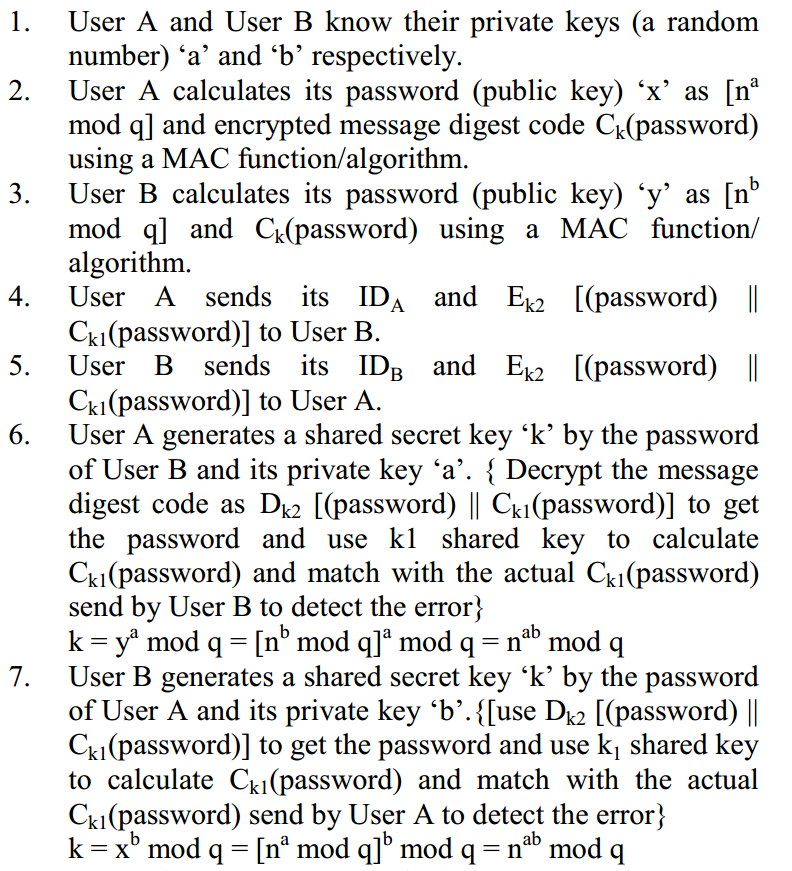
\includegraphics[scale=0.5]{MAC-salasana}

Yhteisenä avaimena toimii siis 'k', jolla toisen osapuolen lähettämä salasana lasketaan. MAC-funktiolla tässä tapauksessa lasketaan salasana julkisille avaimille ja tiiviste salasanalle lähetystä varten.




\subsection{Mobiilikaupankäynti}

Mobiilikaupankäynnillä tarkoitetaan mobiililaitteella tehtäviä maksutransaktioita tai ostotapahtuman vahvistavia viestejä. Menetelmä on siis osa elektronista kaupankäyntiä, jossa käytetään digitaalisia allekirjoituksia \cite{e-c}. Schwab ja Yang toteavat  \cite{enti} suurten datamäärien varastoinnin olevan yleisiä nykyaikaisilla mobiililaitteilla. Samadanin, Shajarin ja Ahanihan artikkelissa \cite{proxy} esitellään huutokauppasovellus, joka vaatii jokaisen huudon varmistuksen lyhyen ajan sisällä laitteella. Allekirjoitusten luonti tulee olla siis nopeaa mobiililaitteilla tietoturva huomioon ottaen. Sekä laite- että palvelinpohjaisia allekirjoituksia käytetään mobiilikaupankäynnissä \cite{proxy}. Verkkopankki, maksusuoritukset, terveydenhoito ja äänestys ovat mahdollisia kannettavilla laitteilla, mutta langaton verkko tuo ongelmansa kaistanleveyden kanssa \cite{ECC}. 



\section{Laitepohjaiset allekirjoitukset}

Mobiililaite koostuu SIM-kortista ja laitteesta, jossa allekirjoituksen luonti tapahtuu prosessorilla. Laitteen käyttöjärjestelmän on tuettava yleisesti käytettyjä protokollia, jotta salaus, tiviisitefunktiot, varmenteet ja digitaaliset allekirjoitukset ovat mahdollisia. Tietoturvan kannalta SIM-korttia voidaan pitää parempana vaihtoehtona, mutta allekirjoitusten luomisen nopeudessa prosessori on tehokkaampi. Salaisen avaimen säilytyspaikka tulee kuitenkin valita turvallisesti, jotta ulkopuolinen tunkeutuja ei saa tietää salaista avainta. Lisäksi on olemassa malli, jossa SIM-kortti ja laitteen prosessori yhdessä osallistuvat allekirjoituksen luontiin (hybridimalli). Seuraavat alaotsikot perustuvat Samadanin, Shajarin ja Ahanihan malleihin \cite{proxy}. 
 
\subsection{SIM-kortilta luonti}

Laitteen SIM-korttia voidaan pitää turvallisimpana paikkana säilyttää salaista avainta. Edes käyttäjä itse tai laitteen käyttöjärjestelmä ei pääse käsiksi salaiseen avaimeen kortilla. Kuitenkin SIM-kortin laskentakapasiteetti on huomattavasti pienempi kuin laitteen prosessorin. Allekirjoituksen luonti SIM-kortilla on erittäin hidasta.   

\subsection{Laitteen prosessorilla luonti}

Salaisen avaimen säilytys voi tapahtua myös laitteen muistissa. Digitaalinen allekirjoitus luodaan tällöin laitteen prosessorilla, joka on laskentateholtaan huomattavasti tehokkaampi kuin SIM-kortti. Käyttöjärjestelmä voi myös tarjota kirjastoja ja työkaluja allekirjoitusten luontiin. Laitteen käyttöjärjestelmässä voi kuitenkin olla tietoturva-aukko, jota hyväksikäyttäen tunkeutujat voivat saada haltuunsa käyttäjän salaisen avaimen.

\subsection{Hybridimalli}

Hybridimallissa salainen avain joudutaan hetkellisesti paljastamaan laitteen käyttöjärjestelmälle. Tässä menetelmässä on siis olemassa pieni tietoturvariski. Hyvänä puolena hybridimallissa on sen lähes yhtä nopea tehokkuus kuin prosessorilla luonnissa. Monet graafisen käyttöliitymän vaativat ohjelmat tarvitsevat prosessorin laskentatehoa, mutta SIM-kortti voi toimia tietoturvan kannalta avaimen yleisenä säilytyspaikkana. Mallissa allekirjoitus siis luodaan prosessorilla, jolloin salaista avainta käytetään vain hetkellisesti laitteessa.


\subsection{Tunnistautuminen laitteella}
Kun käyttäjä haluaa lähettää viestin palvelimelle tai toiselle käyttäjälle, on tärkeää suosia turvallista protokollaa. On turvallista varmistaa myös oikean henkilön käyttävän laitetta, sillä ulkopuolinen varas on voinut anastaa laitteen. Käyttäjän tunnistautuminen voi perustua salasanan syöttämiseen tai visuaaliseen todennukseen. Istunto laitteen ja palvelimen välille voidaan muodostaa Diffien ja Hellmanin protokollaa käyttäen. Viestit salataan yhteisellä avaimella. RSA on kuitenkin parempi välimieshyökkäystä vastaan. 

\subsection{Tunnistautuminen GSM-verkossa}

Verkossa on tärkeää, että viestin lähettäjä tietää lähettävänsä viestin oikealle kohteelle ja vastaanottaja tietää saavansa viestin oikealta lähettäjältä. Jaiswal ja Kumar \cite{cell} esittelevät GSM-verkon toimintaa kahden mobiililaitteen käyttäjän näkökulmasta. Tähän väliin tarvitaan pääsolmu, joka luo yhteisen avaimen osapuolille viestien vaihtoa varten. Verkko voidaan jakaa useampaan kenttään, jossa jokaisessa on oltava vähintään yksi pääsolmu laitteiden tunnistautumista varten. Pääsolmun on tiedettävä kaikki oman kenttänsä laitteet ja muita pääsolmuja tiedon vaihtoa varten. Pääsolmun luo yhteisen avaimen osapuolille tulevaa tiedonvaihtoa varten tunnistetietojen perusteella. Pääsolmu tarvitsee laitteilta tärkeät tiedot tunnistamiseen parametrien ja sijainnin avulla. Tiedonkeruun jälkeen pääsolmu luo yhteisen avaimen osapuolille tulevaa kommunikaatiota varten. Avaimella voi hoitaa viestien salauksen ja tiivisteen käytön.

\section{Palvelinpohjaiset allekirjoitukset}

Palvelin voi luoda digitaalisen allekirjoituksen käyttäjän puolesta, kunhan käyttäjä voidaan todentaa palvelimelle. Palvelinten rooli digitaalisten allekirjoitusten luonnissa oli merkittävä aikana, jolloin laitteissa ei ollut tarpeeksi tehoa allekirjoituksen luomiseen. Nykyään laitepohjaiset allekirjoitukset ovat yleistyneet. \cite{proxy}

\subsection{Välityspalvelin}

Välityspalvelin toimii siis eräänlaisena kirjautumispalvelimena käyttäjän ja lopullisen palveluntarjoajan välissä. Välityspalvelin voi luoda allekirjoituksen, mutta oikean käyttäjän todennus vaaditaan. Varmennus voi perustua algoritmeihin kuten RSA tai DSA. On myös mahdollista, että käyttäjälle tehdään varmenne, jolla hän on tunnistettavissa jatkossa palvelimelle \cite{proxy}.

\subsection{NRS ja NRR}

Kiistämättömyys on olennainen osa digitaalista allekirjoitusta. NRS (Non-Repudation of Sender) tarkoittaa, lähettäjä ei voi jälkikäteen kiistää lähettäneensä viestin. NRR (Non-Repudation of Receiver) puolestaan merkitsee vastaanottajan kiistämättömyyttä. Tiivistefunktioilla varmistetaan datan eheys kuten esimerkiksi MD5:llä. Sekä lähettäjän että vastaanottajan on luotava julkiset avaimet ja merkit kirjautumispalvelimelle tunnistettavaksi. Kirjautumispalvelin pyytää varmenteen varmenneviranomaiselta ja muodostaa oman varmenteen lähettäjälle. Näin ollen kirjautumispalvelin voi jatkossa toimia pysyvämpänä vahvistajana lähettäjän ja vastaanottajan välillä. \cite{gene}

\subsection{Yhdistetty allekirjoitus}

Laitteella pystyy delegoimaan allekirjoituksen luonnin palvelimelle kokonaan, osittain tai valtakirjalla. Välityspalvelin voi kokonaan luoda allekirjoituksen käyttäjän salaisella avaimella. Tämä tyyppi ei ole tietoturvan kannalta suotavaa. Osittaisessa allekirjoituksessa käyttäjä luo omasta salaisesta avaimestaan välityspalvelimelle uuden avaimen. Välityspalvelimella on tällöin mahdollisuus tehdä allekirjoitus käyttäjän puolesta. Kiistattomuus nousee näissä kahdessa menetelmässä ongelmaksi. Vastaanottaja ei voi tietää, onko allekirjoitus tullut välityspalvelimelta vai käyttäjältä. Kolmas menetelmä on valtakirjan luovuttaminen välityspalvelimelle. Käyttäjä siis kertoo valtakirjallaan luovuttaneensa allekirjoitusoikeuden toiselle palvelimelle. Valtakirja luodaan käyttäjän salaisella avaimella. Valtakirjan laatiminen saattaa viedä huomattavasti aikaa ja paljon laskentatehoa. \cite{joint}

\subsection{Tekstiviestitodennus}

Langattomien lähiverkkotekniikoiden yleistymisestä huolimatta tekstiviestillä (SMS) voidaan todentaa käyttäjä. Tarvitaan vain terminaaliemulaattori (T) käyttäjän laitteelle ja turvallinen yhteydenmuodostusportti (GW) kommunikaatiota varten. Terminaali voi olla laitteella erillinen ohjelma tai suoraan integroitu SIM-kortilla oleviin työkaluihin. GW koostuu todennuspalvelimesta ja tietokantapalvelimesta. Todennuspalvelin varmistaa oikean ohjelman käyttävän palvelua ja tietokantapalvelin hallinnoi käyttäjän julkista avainta sekä GW:n salaista avainta.

Seuraavaksi esitelty kuva perustuu Shun, Tanin ja Wangin \cite{sms} tutkimuksiin turvallisesta mobiilikäyttäjän todentamisesta. Sekä T:n että GW:n on luotava tunnistemuuttuja (VF), jolla osapuolet todentavat toisensa. Muuttuja voi olla esimerkiksi tietyn pituinen tiiviste, joka perustuu satunnaislukuihin. Lähtevät paketit luonnollisesti salataan. Oletetaan tiivisteen nimeksi vaikka Nc. Terminaali tekee yhteydenmuodostuspyynnön REQ1, jossa on mukana Nc. GW tutkii pyynnön ja tarkistaa käyttäjän identiteetin sekä puhelinnumeron. Tietokantakyselyllä GW varmistaa käyttäjän löytyvän tietokannasta. GW luo oman VF:n nimeltä Ns ja istuntoavaimen nimeltä Ks. Nämä molemmat muuttujat sekä aiemman Nc:n GW allekirjoittaa salaisella avaimellaan. ACK1-vastauksessa GW hyväksyy yhteydenmuodostuksen ja lähettää salatussa muodossa Nc:n, Ns:sän ja Ks:sän. Tämän jälkeen T:llä allekirjoitetaan saapunut ACK1-vastaus käyttäjän salaisella avaimella. Jos allekirjoitettu Nc' on sama kuin käyttäjän alunperin lähettämä Nc-muuttuja, T salaa Ks:sän ja Ns:sän uudessa pyyntöviestissä REQ2 ja hoitaa lähetyksen. Nyt puolestaan GW allekirjoittaa Ns:n. Mikäli Ns' on sama kuin alunperin lähetetty Ns, yhteys käyttäjän ja palvelimen välille on luotu ja GW lähettää terminaalille kuittauksen ACK2 yhteydenmuodostuksen onnistumisesta. Alla oleva kuva kertoo tarkemmin protokollasta.   

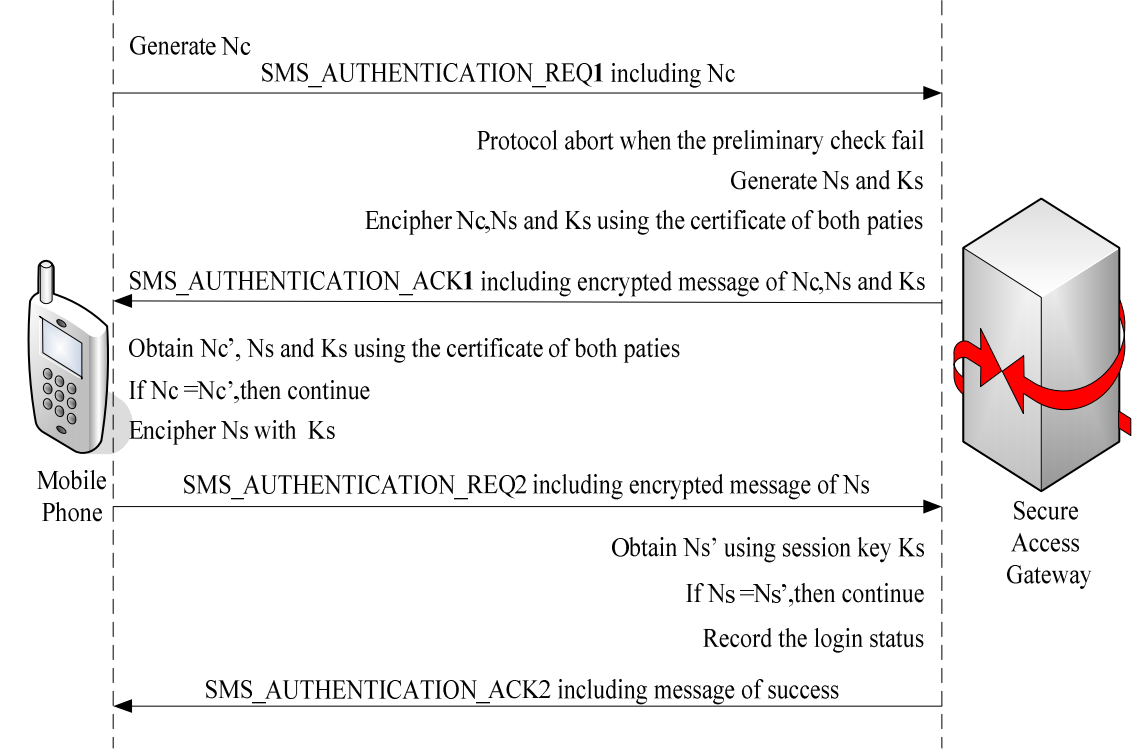
\includegraphics[scale=0.4]{sms-todennus}

Koska protokolla perustu satunnaisiin muuttujiin, se on resistanssi välimieshyökkäykselle. Myös kiistämättömyys luodaan, sillä käyttäjän salainen avain säilyy vain laitteessa ja terminaali käyttää avainta. Tätä kyseistä protokollaa voidaan siis pitää yhdistettynä mallina palvelin- ja laitepohjaisesta allekirjoituksesta.


\subsection{Varmenteet}

Varmenteet ovat kolmannen osapuolen antaman varmenneviranomaisen todistuksia. Myös välityspalvelin voi luoda varmenteen käyttäjälle \cite{proxy}. Jokin käyttäjä, välityspalvelin tai lopullinen palveluntarjoaja tarvitsee varmenteen jatkuvaa yhteydenpitoa varten, koska varmenne kuuluu digitaalisen allekirjoituksen protokollaan. Varmenne voi olla voimassa päiviä, kuukausia tai vuosia, mutta tietoturvan kannalta varmenteiden ei tulisi olla ikuisia. Varmennetta voidaan pitää luotettavana, jos sen tarjoaa ulkopuolinen varmenneviranomainen. Digitaalinen allekirjoitus vaatii toimiakseen aina varmenteen, mutta varmenne voi toimia irrallisena digitaalisesta allekirjoituksesta esimerkiksi palvelinten välisessä tunnistuksessa \cite{proxy}. PKI-protokollan avulla varmenne voidaan luoda luovuttamalla julkinen avain varmenneviranomaiselle ja lähettämällä varmennepyyntö. Tämän jälkeen käyttäjä vahvistaa vielä itsensä salaamalla viestinsä salaisella avaimellaan. Varmenneviranomainen vastaa luovuttamalla varmenteen käyttäjälle. Varmenteeseen on yleensä merkitty seuraavat tiedot: voimassaoloaika, sarjanumero, versio ja käyttäjän tunniste \cite{ECC}. Vastaanottajan tulee siis ottaa huomioon vanhentunut varmenne. Koska varmenne on yksilökohtainen, hyökkääjä ei tee varastetulla varmenteella mitään. 

\section{Vertailu}

Tehokkuus ja tietoturva ovat tärkeitä ominaisuuksia koskien digitaalisia allekirjoituksia. Vaikka nämä kaksi seikkaa eivät ole suoraan toisensa poissulkevia, on syytä ottaa huomioon kummankin prioriteetti. Erityisesti mobiililaitteilla tehokkuudesta joudutaan yleensä karsimaan, joten valitaan vähemmän tehokas allekirjoitusalgoritmi. Tällöin allekirjoittaminen on hidas prosessi \cite{proxy}.

\subsection{Tietoturva}

Mobiililaitteilla voidaan havaita seuraavia tietoturvariskejä: urkinta, välimieshyökkäys, datan muuntaminen, toisena osapuolena esiintyminen ja laitteen kadottaminen. Urkinnalla tarkoitetaan viestien kuuntelua, mutta se voidaan torjua helposti viestin salakirjoituksella esimerkiksi väliaikaisella istuntoavaimella. Välimieshyökkäys tarkoittaa kolmannen osapuolen asettumista lähettävän ja vastaanottavan osapuolten väliin. DH:ssa voi piileä tämä riski mutta ei yleensä RSA:ssa \cite{enti}. Datan muuntaminen voidaan estää salakirjoituksella sekä käyttämällä tiivistefunktioita. Toisena osapuolena tekeytyminen ja laitteen kadottaminen voidaan estää salasanan kirjoittamisella laitteelle tai visuaalisella todennuksella. 

Julkisen avaimen infrastruktuuri eli PKI-malli toimii, jos salainen avain säilyy suojassa. Mikäli on pienikin riski, että salainen avain on jokun muun tiedossa tulee avainpari vaihtaa heti. Niin kauan kun diskreetin logaritmin ongelmaa ei pystytä ratkaisemaan järkevässä ajassa, ovat RSA ja DH turvallisia protokollia. Tiivistefunktioiden tulee olla myös ajan tasalla, jotta allekirjoitusten salaus toimii. Esimerkiksi tulevaa SHA-3 standardia kehitellään paremmaksi tulevaa käyttöönottoa varten \cite{nist}.
	  

\subsection{Tehokkuus}

Suorituskyky on parantunut vuosien saatossa niin tietokoneilla kuin mobiililaitteilla. Prosessorien teknologia on kehittynyt mahdollistaen tiheämmät kellopulssit ja moniydinsuorituksen. Myös tietoliikennenopeuksien kasvamisella on ollut suuri merkitys digitaalisten allekirjoitusten luonnissa. Tehokkuutta tarvitaan nopeisiin allekirjoituksiin lyhyellä aikavälillä. Artikkelissa Self-Proxy Mobile Signature \cite{proxy} esitelty huutokauppasovellus tarvitsee jokaiselle huudolle uuden  allekirjoituksen lyhyen ajan sisällä. Tietoturvasta on tässä tapauksessa erittäin vaikea tinkiä, joten käyttäjän olisi hyvä luoda allekirjoitus omalta laitteeltaan. Tehokkuudessa tulee ottaa huomioon siis salauksen nopeus, tiivisteen luominen ja varmenteen hankinta \cite{proxy}. Luonnollisesti myös palvelinpuolella esimerkiksi klusterointi on luonut mahdollisuuden tehokkaaseen allekirjoitusten/varmenteiden luomiseen monelle käyttäjälle samaan aikaan.

\subsection{Nykyaikaisten menetelmien käyttö}

Laitepohjaiset allekirjoitukset ovat vakiintuneet kokoajan mobiililaitteiden laskentatehon kasvun ansiosta. RSA:n lisäksi elliptiset käyrät ovat yleistyneet niiden paremman tietoturvan ansiosta suhteessa avainten pituuteen bitteinä \cite{ECC}. AES algoritmia voidaan pitää murtumattomana, mutta DSA on murrettavissa jo muutaman bittivuodon avulla \cite{gsm}. Elliptisen käyrän DSA:ta käytetään myös mobiililaitteilla \cite{webs}. RSA:n avaimen pituuden on hyvä olla vähintään 1024 bittiä. Elliptisissä käyrissä riittää 160 bittiä tällä hetkellä \cite{ECC}.

Android-käyttöjärjestelmä tukee Javan virtuaalikonetta (JVM). Java käyttää digitaaliseen allekirjoitukseen tarvittavia protokollia, joita tarvitaan monilla mobiililaitteilla nykypäivänä. Bouncy Castle- paketti tarjoaa Javassa monenlaista kryptografisia algoritmeja tiedon salaukseen ja purkamiseen. Javalla myös satunnaisten olioiden luominen on helppoa. \cite{enti}   

\section{Yhteenveto}  

Tässä tekstissä olemme tarkastelleet digitaalisia allekirjoituksia mobiiliympäristöissä ja mobiililaitteissa. Digitaalisen allekirjoituksen ehtoina ovat vastaanottajan todennus, datan eheys ja lähettäjän kiistämättömyys. Menetelmät allekirjoitusten luontiin vastaavat tietokoneilla samanlaisia menetelmiä. Olemme tarkastelleet julkisen avaimen infrastruktuuria, RSA:n ja Diffien ja Hellmanin menetelmää tarkemmin sekä mobiilikaupankäyntiä. Digitaalisten allekirjoitusten luonti voidaan jakaa kahteen pääryhmään: laite- ja palvelinpohjaisiin allekirjoituksiin. Laiteella allekirjoituksen voi luoda prosessori tai SIM-kortti. Lisäksi hybridimallin olemassaolo tunnetaan. Palvelinpuolella tulee korostua käyttäjän tunnistaminen ja kirjautumispalvelimen merkitys. Kiistattomuuden tulee toimia delegoinnin yhteydessä. Digitaalinen allekirjoitus voidaan delegoida palvelimelle kokonaan, osittain tai valtakirjalla. Varmenteet ja kiistattomuus luovat digitaalisen allekirjoituksen pohjan. Olemme tarkastelleet tekstin lopussa tietoturvan ja tehokkuuden merkitystä digitaalisissa allekirjoituksissa mobiiliympäristö huomioon ottaen. Nykyaikaisiin menetelmiin voimme luetella RSA:n, DSA:n, DH:n ja elliptisten käyrien algoritmit, joita muun muassa Android-käyttöjärjestelmä tukee.


% --- References ---
%
% bibtex is used to generate the bibliography. The babplain style
% will generate numeric references (e.g. [1]) appropriate for theoretical
% computer science. If you need alphanumeric references (e.g [Tur90]), use
%
% bibliographystyle{babplain-lf}
%
% instead.

\newpage
\bibliographystyle{babalpha-lf}
\bibliography{viitteet}


% --- Appendices ---

% uncomment the following

%\newpage
%\appendix
 
%\section{Esimerkkiliite}

\end{document}